\documentclass[10pt]{ctexart}
\usepackage{morelull}
\usepackage{enumerate}
\usepackage{bm}
\usepackage{makecell}
\usepackage{xcolor}
\usepackage{graphicx}
\usepackage{subfigure}
\usepackage{framed}%包中有添加文字背景色命令shaded
\colorlet{shadecolor}{MaterialBlue50}
\usepackage{tabularx}
\usepackage{multicol}  
\usepackage{multirow}
\usepackage{indentfirst}
\usepackage{amsmath,amssymb,amsthm,bm,bbding,pifont,dsfont}
\usepackage{mathtools}
\newcommand{\abs}[1]{\left| #1 \right|}
\usepackage{caption}
\captionsetup[figure]{labelfont={bf},labelformat={default},labelsep=period,name={图}}
%定义选择题选项
\newcommand{\onech}[4]{
\renewcommand\arraystretch{1.4}
\begin{tabularx}{\linewidth}{XXXX}
\setlength\tabcolsep{0pt}
(A) #1 & (B) #2 & (C) #3 & (D) #4 \\
\end{tabularx}
\unskip \unskip}
\newcommand{\twoch}[4]{
\renewcommand\arraystretch{1.4}
\begin{tabularx}{\linewidth}{XX}
\setlength\tabcolsep{0pt}
(A) #1 & (B) #2 \\
(C) #3 & (D) #4
\end{tabularx}
\unskip \unskip}

\title{模型研究系列 \quad 角平分线交角模型}
\author{一粒沙整理\\安徽省霍邱县龙潭中心校}
\date{\today}



\begin{document}
\maketitle
\tableofcontents


\section{知识储备:与中点有关的概念}
{\kaishu\color{blue}
\begin{enumerate}
	\item {\heiti\color{cyan}三角形中线的定义}:三角形顶点和对边中点的连线.
	\item {\heiti\color{cyan}三角形中线的相关定理}:直角三角形斜边的中线等于斜边的一半;
等腰三角形底边的中线三线合一(底边的中线、顶角的角平分线、底边的高重合).
	\item {\heiti\color{cyan}三角形中位线定义}:连结三角形两边中点的线段叫做三角形的中位线.
	\item {\heiti\color{cyan}三角形中位线定理}:三角形的中位线平行于第三边并且等于它的一半.
	\item {\heiti\color{cyan}中位线判定定理}:经过三角形一边中点且平行于另一边的直线必平分第三边.
	\item {\heiti\color{cyan}直角三角形斜边中线}:直角三角形斜边中线等于斜边的一半.
	\item {\heiti\color{cyan}斜边中线判定}:若三角形一边上的中线等于该边的一半,则这个三角形是直角三角形.
\end{enumerate}
}

\section{中点有关的模型}
\subsection{倍长中线或类倍长中线( 与中点有关的线段)构造全等三角形}
【 {\heiti 模型基础}】

\begin{center}
	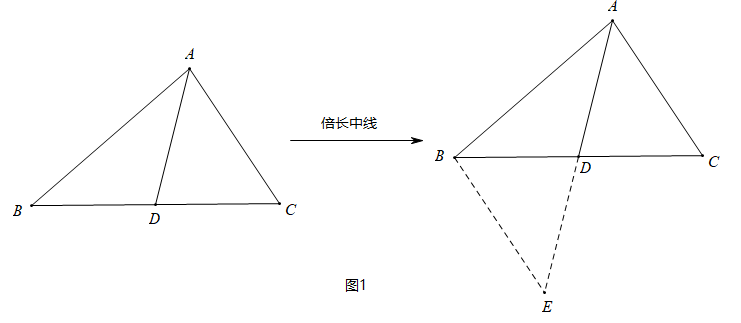
\includegraphics[scale=0.6]{figure/zhongdian01}\\
	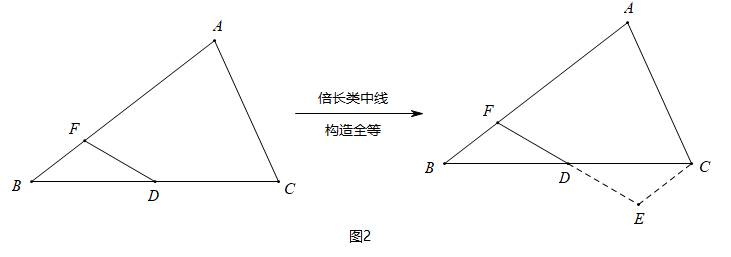
\includegraphics[scale=0.6]{figure/zhongdian02}
\end{center}

【 {\heiti 模型分析}】

如图1,$AD$是$\triangle ABC$的中线,延长$AD$至点$E$使$DE=AD$,易证:$\triangle ADC\cong \triangle EDB(SAS)$.如图2,$D$是$BC$中点,延长$FD$至点$E$使$DE=FD$,易证:$\triangle FDB\cong EDC(SAS)$.

当遇见中线或者中点的时候,可以尝试倍长中线或类中线,构造全等三角形,目的是对已知条件中的线段进行转移。

换个马甲也要认识哦,如下情形中$F$为$DE$的中点,请自证.

\begin{center}
	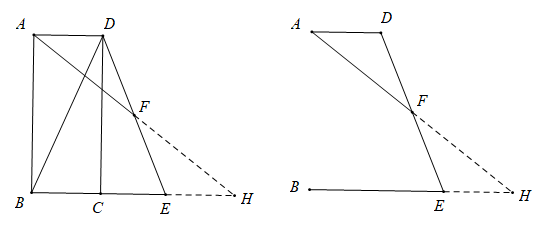
\includegraphics[scale=0.6]{figure/zhongdian03}
\end{center}

点评:
(1)倍长中线:即延长三角形的中线,使得延长后的线段是原中线的两倍.
(2)其目的是构造一对对顶的全等三角形;
(3)其本质是转移边和角.



难点:有些几何题在利用“倍长中线”证完一次全等三角形后,还需要再证一次全等三角形,即“二次全等”。在证明第二次全等时,难点通常体现在倒角上,常见的倒角方法有:\ding{192}“8”字型;\ding{193}平行线;\ding{194}180°(平角、三角形内角和);\ding{195}360°(周角、四边形内角和);\ding{196}小旗子( 三角形外角);\ding{197}90°( 互余角).


【 {\heiti 模型实例}】
\begin{shaded}
	\begin{example}
 	如图,已知在$\triangle ABC$中,$AD$是$BC$边上的中线,$E$是$AD$上一点,连接 $BE$并延长$AC$于点$F$,$AF=EF$。求证:$AC=BE$。
	\end{example}
\end{shaded}

\begin{flushright}
	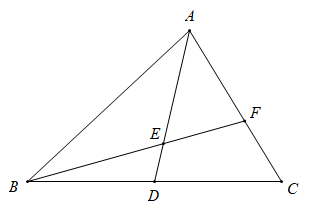
\includegraphics[scale=0.6]{figure/zhongdian04}
\end{flushright}


【 {\heiti 模型精炼}】
\begin{shaded}
	1.如图,在$\triangle ABC$中,$AB=12$,$AC=20$,求$BC$边上中线$AD$的范围。
\end{shaded}

\begin{flushright}
	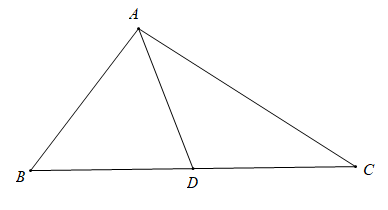
\includegraphics[scale=0.6]{figure/zhongdian05}
\end{flushright}

\begin{shaded}
  	2.如图,在$\triangle ABC$中,$D$是$BC$的中点,$DM\perp DN$,如果$BM^2+CN^2=DM^2+DN^2$。求证:$AD^2=\dfrac{1}{4}\left(AB^2+AC^2\right)$。
\end{shaded}

\begin{flushright}
	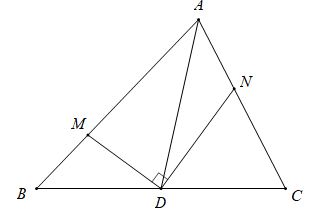
\includegraphics[scale=0.6]{figure/zhongdian06}
\end{flushright}


\subsection{已知等腰三角形底边中点,可与顶点连接用“三线合一”}

【 {\heiti 模型基础}】

\begin{center}
	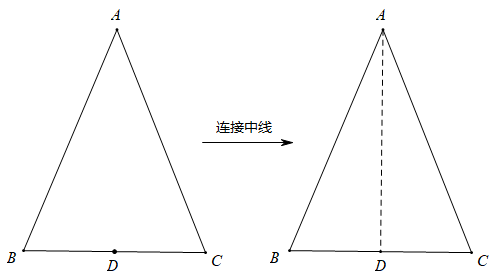
\includegraphics[scale=0.6]{figure/zhongdian07}
\end{center}

【 {\heiti 模型分析}】

等腰三角形中有底边中点时,常作底边的中线,利用等腰三角形“三线合一”的性质得到角相等或边相等,为解题创造更多的条件,当看见等腰三角形的时候,就应想到:“边等、角等、三线合一”。

【 {\heiti 模型实例}】

如图,在$\triangle ABC$中,$AB=AC=5$,$BC=6$,$M$为$BC$的中点,$MN\perp CC$于点$N$, 求$MN$的长度。

\begin{flushright}
	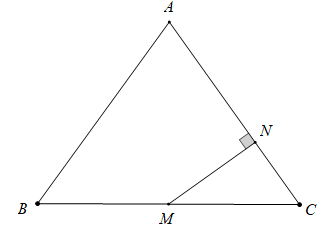
\includegraphics[scale=0.6]{figure/zhongdian08}
\end{flushright}

【 {\heiti 模型精炼}】
\begin{shaded}
1.如图,在$\triangle ABC$中,$AB=AC$,$D$是$BC$的中点,$AE\perp DE$,$AF\perp DF$,且$AE=AF$。求证:$∠\angle EDB=\angle FDC$.
\end{shaded}

\begin{flushright}
	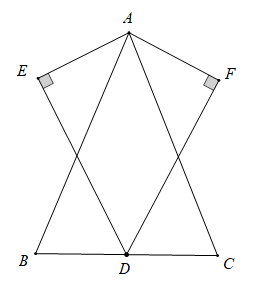
\includegraphics[scale=0.6]{figure/zhongdian09}
\end{flushright}

\begin{shaded}
2.已知$Rt\triangle ABC$中,$AC=BC$,$\angle C=90^\circ$,$D$为$AB$边的中点,$\angle EDF=90^\circ$,$\angle EDF$绕点$D$旋转,它的两边分别交$AC,CB$(或它们的延长线)于$E,F$.

(1)当$\angle EDF$绕点$D$旋转到$DE\perp AC$于$E$时(如图1),
求证:$S_{\triangle DEF}+S_{\triangle CEF}=\dfrac{1}{2}S_{\triangle ABC}$;

(2)当$\angle EDF$绕点$D$旋转到$DE$和$AC$不垂直时,在图2和图3这两种情况下,上述结论是否成立?若成立,请给予证明;若不成立,$S_{\triangle DEF},S_{\triangle CEF},S_{\triangle ABC}$又有怎样的数量关系?请写出你的猜想,不需证明。
\end{shaded}

\begin{flushright}
	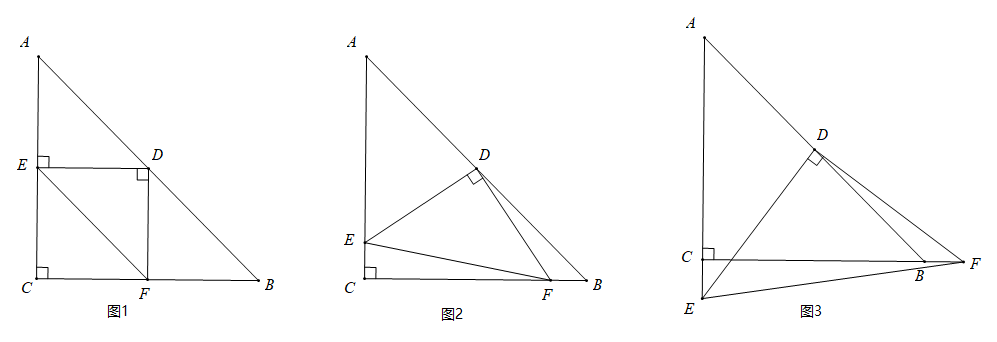
\includegraphics[scale=0.6]{figure/zhongdian10}
\end{flushright}

\subsection{已知三角形一边的中点,可考虑中位线定理}

【 {\heiti 模型基础}】

\begin{center}
	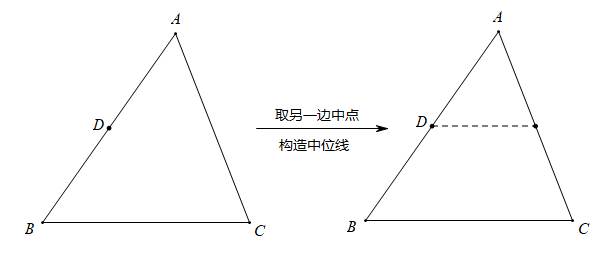
\includegraphics[scale=0.6]{figure/zhongdian11}
\end{center}

【 {\heiti 模型分析}】

	在三角形中,如果有中点,可构造三角形的中位线,利用三角形中位线的性质定理:$DE//BC$,且$DE= \dfrac{1}{2}BC$来解题.中位线定理中既有线段之间的位置关系又有数量关系,该模型可以解决角问题,线段之间的倍半、相等及平行问题.


【 {\heiti 模型实例}】
\begin{shaded}
如图,在四边形$ABCD$中,$AB=CD$,$E,F$分别是$BC,AD$的中点,连接$EF$并延长,分别与$BA,CD$的延长线交于点$M,N$.求证:$\angle BME=\angle CNE$.
\end{shaded}

\begin{center}
	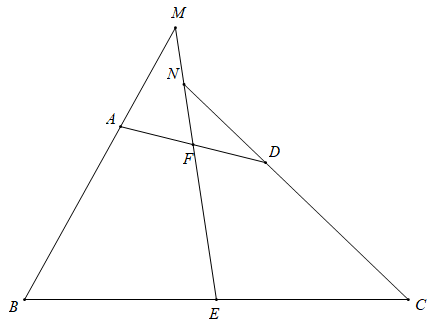
\includegraphics[scale=0.6]{figure/zhongdian12}
\end{center}

【 {\heiti 模型精炼}】

\begin{shaded}
1.(1)如图1,$BD,CE$分别是$\triangle ABC$的外角平分线,过点$A$作$AD\perp BD,
AE\perp CE$,垂足分别为$D,E$,连接$DE$.
求证:$DE//BC$,$DE=\dfrac{1}{2}(AB+BC+AC)$;

(2)如图2,$BD,CE$分别是$\triangle ABC$的内角平分线,其它条件不变。上述结论是否成立? 

(3)如图3,$BD$是$\triangle ABC$的内角平分线,$CE$是$\triangle ABC$的外角平分线,其它条件不变。$DE$与$BC$还平行吗?它与$\triangle ABC$三边又有怎样的数量关系?请写出你的猜想,并对其中一种情况进行证明。 
\end{shaded}

\begin{center}
	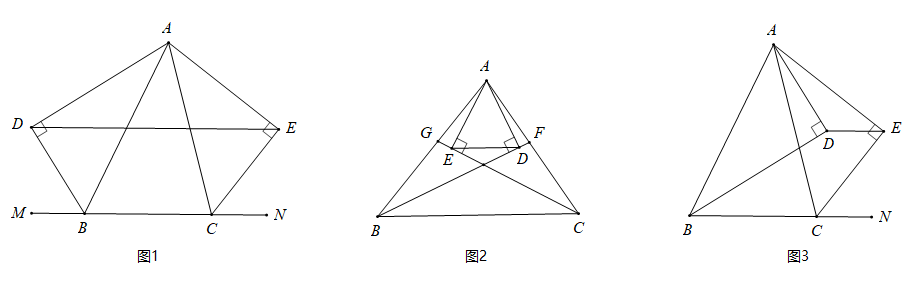
\includegraphics[scale=0.6]{figure/zhongdian13}
\end{center}

\begin{shaded}
2.问题一:如图1,在四边形$ACBD$中,$AB$与$CD$相交于点$O$,$AB=CD$,$E,F$分别是$BC,AD$的中点,连接$EF$分别交$DC,AB$于点$M,N$,判断$\triangle OMN$的形状,请直接写出结论;

问题二:如图2,在$\triangle ABC$中,$AC>AB$,点$D$在$AC$上,$AB=CD$,$E,F$分别是$BC,
AD$的中点,连接$EF$并延长,与$BA$的延长线交于点$G$,若 $\angle EFC=60^\circ$,
连接$GD$,判断$\triangle AGD$的形状并证明。
\end{shaded}

\begin{center}
	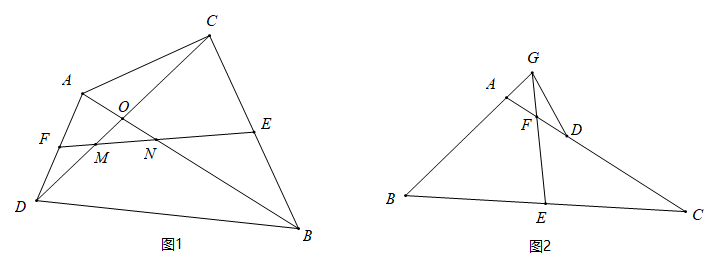
\includegraphics[scale=0.6]{figure/zhongdian14}
\end{center}




\subsection{已知直角三角形斜边中点,可以考虑构造斜边中线}

【 {\heiti 模型基础}】

\begin{center}
	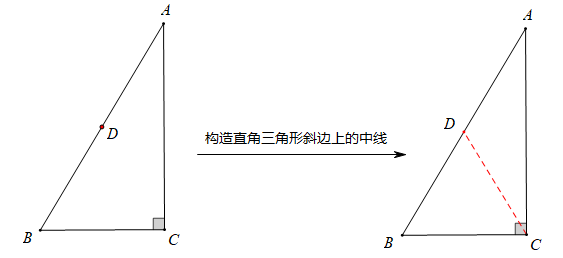
\includegraphics[scale=0.6]{figure/zhongdian15}
\end{center}

【 {\heiti 模型分析}】

在直角三角形中,当遇见斜边中点时,经常会作斜边上的中线,利用直
角三角形斜边上的中线等于斜边的一半,即$CD=\frac{1}{2}AB$,来证明线段间的数量关系,而且可以得到两个等腰三角形:$\triangle ACD$和$\triangle BCD$,该模型经常会与中位线定理一起综合应用。


【 {\heiti 模型实例}】

\begin{shaded}
如图,在$\triangle ABC$中,$BE,CF$分别为$AC,AB$上的高,$D$为$BC$的中点,$DM\perp EF$于点$M$。求证:$FM=EM$。
\end{shaded}

\begin{flushright}
	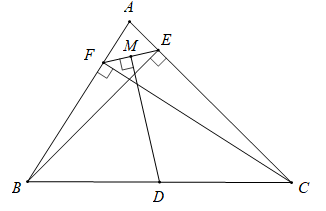
\includegraphics[scale=0.6]{figure/zhongdian16}
\end{flushright}

【 {\heiti 模型精炼}】

\begin{shaded}
1.如图,在$\triangle ABC$中,$\angle B=2\angle C$,$AD\perp BC$于点$D$,$M$为$BC$的中点,$AB=10$。求$DM$的长度。
\end{shaded}

\begin{flushright}
	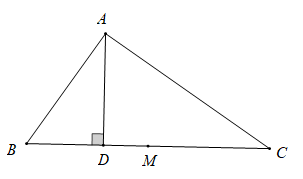
\includegraphics[scale=0.6]{figure/zhongdian17}
\end{flushright}

\begin{shaded}
2.已知,$\triangle ABD$和$\triangle ACE$都是直角三角形,且$\angle
 ABD=\angle ACE=90^\circ$,连接$DE$,$M$为$DE$的中点,连接$MB,MC$。求证:$MB=MC$。
\end{shaded}

\begin{flushright}
	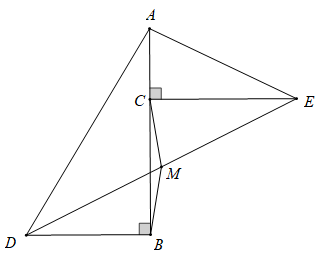
\includegraphics[scale=0.6]{figure/zhongdian18}
\end{flushright}

\begin{shaded}
3.问题1:如图1,,$\triangle ABC$中,点$D$是$AB$边的中点,$AE\perp BC$,$BF\perp AC$,垂足分别为点$E,F$,$AE,BF$交于点$M$,连接$DE,DF$。若$DE=kDF$,则$k$的值为$\underline{\hspace{1.5cm}}$;

问题2:如图2,,$\triangle ABD$中,$CB=CA$,点$D$是$AB$边的中点,点$M$在,$\triangle ABD$内部,且$\angle MAC=\angle MBC$。过点$M$分别作$ME\perp BC$,$MF\perp AC$,垂足分别为点$E,F$,连接$DE,DF$。若$DE=DF$;

问题3:如图3,若将上面问题2中的条件$CB=CA$变为$CB\neq CA$,其它条件不变,试探究$DE$与$DF$之间的数量关系,并证明你的结论。
\end{shaded}

\begin{center}
	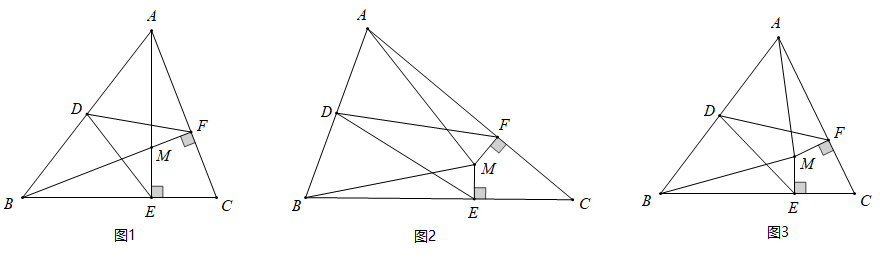
\includegraphics[scale=0.6]{figure/zhongdian19}
\end{center}



\end{document}